% =====================================================================
%  Academic Internship Report: StudyPilot
%  Ayushman Lahon, Roll No. 2481102474, B.Tech CSE, 5th Semester
%  Compile with pdfLaTeX (Overleaf default) or Tectonic.
%  Images are expected in the folder  figures/
% =====================================================================
\documentclass[12pt,a4paper]{report}

% ---------- Fonts and page ----------
\usepackage[T1]{fontenc}
\usepackage{newtxtext,newtxmath}          % Times-like text and maths
\usepackage[scaled=0.92]{inconsolata}      % typewriter font for code and URLs
\usepackage[a4paper,top=2.3cm,bottom=2.3cm,left=2.7cm,right=2.3cm,headheight=15pt]{geometry}
\usepackage{setspace}
\setstretch{1.12}
\usepackage{microtype}

% ---------- Colours, figures, tables ----------
\usepackage{xcolor}
\definecolor{navy}{RGB}{31,56,120}
\definecolor{boxfill}{RGB}{232,238,250}
\definecolor{softgrey}{RGB}{245,245,247}
\usepackage{graphicx}
\graphicspath{{figures/}}
\usepackage{float}
\usepackage{wrapfig}
\usepackage{caption}
\usepackage{subcaption}
\captionsetup{labelfont={bf,color=navy},font=small,labelsep=colon,skip=5pt}
\usepackage{booktabs}
\usepackage{tabularx}
\usepackage{array}
\newcolumntype{L}{>{\raggedright\arraybackslash}X}
\newcolumntype{P}[1]{>{\raggedright\arraybackslash}p{#1}}   % left-aligned fixed-width column
\usepackage{enumitem}
\setlist{itemsep=1pt,topsep=3pt}
\usepackage{tikz}
\usetikzlibrary{positioning,arrows.meta,fit,calc,shapes.geometric}

% ---------- Headings ----------
\usepackage{titlesec}
\titleformat{\chapter}[display]
  {\normalfont\bfseries\color{navy}}
  {\scshape\large Chapter \thechapter}{2pt}{\Huge}
  [\vspace{2pt}{\color{black}\titlerule}]
\titleformat{name=\chapter,numberless}[block]
  {\normalfont\bfseries\color{navy}}{}{0pt}{\Huge}
  [\vspace{4pt}{\color{black}\titlerule}]
\titlespacing*{\chapter}{0pt}{0pt}{14pt}
\titleformat{\section}{\normalfont\Large\bfseries\color{navy}}{\thesection}{0.8em}{}
\titlespacing*{\section}{0pt}{12pt}{4pt}
\titleformat{\subsection}{\normalfont\large\bfseries\color{navy}}{\thesubsection}{0.8em}{}

% ---------- Header and footer ----------
\usepackage{fancyhdr}
\pagestyle{fancy}
\fancyhf{}
\fancyhead[L]{\small\itshape Academic Internship Report}
\fancyhead[R]{\small\itshape\nouppercase{\leftmark}}
\fancyfoot[C]{\thepage}
\renewcommand{\headrulewidth}{0.4pt}
\renewcommand{\chaptermark}[1]{\markboth{Chapter \thechapter.\ #1}{}}
\fancypagestyle{plain}{\fancyhf{}\fancyfoot[C]{\thepage}\renewcommand{\headrulewidth}{0pt}}

% ---------- Links ----------
\usepackage{xurl}
\usepackage[hidelinks]{hyperref}

% ---------- Small helpers ----------
\newcommand{\code}[1]{\texttt{#1}}
\tikzset{
  blk/.style={draw=navy!70,fill=boxfill,rounded corners=2pt,align=center,
              font=\small,minimum height=0.95cm,inner sep=4pt},
  plain/.style={draw=black!40,fill=white,rounded corners=2pt,align=center,
                font=\small,minimum height=0.95cm,inner sep=4pt},
  arr/.style={-{Stealth[length=2.2mm]},thick,black!65},
  grp/.style={draw=black!35,dashed,rounded corners=4pt,inner sep=7pt},
  grplabel/.style={font=\small\bfseries,text=navy,anchor=south west}
}

\renewcommand{\bibname}{References}
\begin{document}

% =====================================================================
%  TITLE PAGE
% =====================================================================
\begin{titlepage}
\begin{tikzpicture}[remember picture,overlay]
  \draw[navy,line width=1.6pt]
    ($(current page.north west)+(1.2cm,-1.2cm)$) rectangle
    ($(current page.south east)+(-1.2cm,1.2cm)$);
  \draw[navy!60,line width=0.4pt]
    ($(current page.north west)+(1.4cm,-1.4cm)$) rectangle
    ($(current page.south east)+(-1.4cm,1.4cm)$);
\end{tikzpicture}
\centering
\vspace*{0.4cm}

% College logo, then the college and department

\includegraphics[width=2.6cm]{jec-logo.jpg}\\[12pt]
{\color{navy}\LARGE\bfseries Jorhat Engineering College}\\[4pt]
{\small Department of Computer Science and Engineering}\\[30pt]

{\color{navy}\large\bfseries\scshape An Academic Internship Report}\\[14pt]
{\color{navy}\rule{0.85\textwidth}{0.8pt}}\\[16pt]
{\color{navy}\fontsize{34}{40}\selectfont\bfseries StudyPilot}\\[12pt]
{\Large A Personal AI Study Assistant\\[2pt]
using RAG and LLMs}\\[12pt]
{\color{navy}\rule{0.85\textwidth}{0.8pt}}\\[30pt]

{\small Done through the Udemy course}\\[4pt]
{\large\itshape AI Engineer Core Track: LLM Engineering, RAG, QLoRA, Agents}\\[2pt]
{\small by Ed Donner (July--August 2026)}\\[30pt]

{\small\bfseries Submitted by}\\[8pt]
\fbox{\begin{minipage}{0.5\textwidth}\vspace{6pt}
\small
\begin{tabular}{@{\hspace{6pt}}l@{\hspace{14pt}}l}
Name      & \textbf{Ayushman Lahon} \\
Roll No.  & 2481102474 \\
Programme & B.Tech, CSE \\
Semester  & 5th \\
Batch     & 2024--28 \\
\end{tabular}
\vspace{6pt}\end{minipage}}\\[30pt]

{\color{navy}\bfseries Academic Session 2026--27}
\end{titlepage}

% =====================================================================
%  FRONT MATTER
% =====================================================================
\pagenumbering{roman}
\setcounter{page}{2}

% ---------- Certificate ----------
\chapter*{Course Completion Certificate}
\addcontentsline{toc}{chapter}{Course Completion Certificate}
I finished the course on \textbf{4 August 2026}. The certificate given by Udemy is shown below.

\vspace{10pt}
\begin{center}
\fcolorbox{black!25}{white}{
\includegraphics[width=0.86\textwidth]{certificate.jpg}}
\end{center}
\vspace{14pt}
\begin{center}
\small
\begin{tabularx}{0.86\textwidth}{@{}lL@{}}
\toprule
Certificate No.    & UC-70a45f64-725c-40d4-93d2-48a4fa1d74ad \\
Verify at          & \url{https://ude.my/UC-70a45f64-725c-40d4-93d2-48a4fa1d74ad} \\
Course length      & 33.5 total hours \\
Instructors        & Ligency, Ed Donner \\
Date of completion & 4 August 2026 \\
\bottomrule
\end{tabularx}
\end{center}

% ---------- Declaration ----------
\chapter*{Declaration}
\addcontentsline{toc}{chapter}{Declaration}
I, \textbf{Ayushman Lahon}, a 5th semester student of B.Tech in Computer Science and
Engineering (Batch 2024--28) at Jorhat Engineering College, Roll No.\ 2481102474, declare
that this academic internship report titled ``StudyPilot: A Personal AI Study Assistant
using RAG and LLMs'' is a record of my own work. The internship was done in
July and August 2026 through the online course ``AI Engineer Core Track: LLM Engineering,
RAG, QLoRA, Agents'' on Udemy.

The project described here was planned and built by me. This report has not been
submitted to any other university or institution for any degree or diploma. Wherever I
have used the work of others, I have mentioned it in the references.

\vspace{2.2cm}
\noindent
\begin{minipage}[t]{0.45\textwidth}
Place: Jorhat\\[6pt]
Date:
\end{minipage}\hfill
\begin{minipage}[t]{0.45\textwidth}\raggedleft
(Ayushman Lahon)\\
Roll No.: 2481102474
\end{minipage}

% ---------- Acknowledgement ----------
\chapter*{Acknowledgement}
\addcontentsline{toc}{chapter}{Acknowledgement}
I want to thank everyone who helped me during this internship.

First, I thank the \textbf{Department of Computer Science and Engineering, Jorhat
Engineering College}, for making the academic internship a part of our course and for
letting us choose an area we really want to learn.

I am very thankful to \textbf{Mr.\ Ed Donner}, the instructor of ``AI Engineer Core Track:
LLM Engineering, RAG, QLoRA, Agents''. Every week of his course ends with something that
actually works, so I was always building and not only watching. His explanation that an
LLM has no memory of its own, and that the program has to send the conversation again
every time, changed how I think about chat applications.

I also thank the people who build and maintain the free tools I used, like FastAPI, React,
ChromaDB, Ollama, EasyOCR and PyMuPDF, the Qwen team for their open models, and Google for
the free tier of the Gemini API. Their documentation helped me a lot when I got stuck.

Lastly, I thank my parents, teachers and friends for their support and patience during
this time.

\vspace{1.6cm}
\begin{flushright}
\textbf{Ayushman Lahon}\\
Roll No.: 2481102474
\end{flushright}

% ---------- Abstract ----------
\chapter*{Abstract}
\addcontentsline{toc}{chapter}{Abstract}
This report covers my academic internship, done in July and August 2026 through the
33.5-hour Udemy course ``AI Engineer Core Track: LLM Engineering, RAG, QLoRA, Agents'' by
Ed Donner.

The first part of the report is about the course. It taught how to call Large Language
Models (LLMs) through their APIs, how to run open-source models on my own computer, how to
choose a model for a task, how to build Retrieval-Augmented Generation (RAG) systems with
embeddings and a vector database, how to fine-tune models with LoRA and QLoRA, and how
several LLM calls and tools can work together as agents.

The second part is about \textbf{StudyPilot}, a web application I built using these ideas.
A student adds their own study material: lecture PDFs, scanned notes or photos (read with
OCR), and YouTube lectures (read from their transcripts). They can then chat with this
material and get answers that cite the file and page, revise with flashcards that come back
on a spaced-repetition schedule, and take quizzes that are graded with feedback. If a
question is not about the uploaded material, the assistant notices this and answers
normally instead of forcing an answer from unrelated pages.

The backend uses Python and FastAPI, and the frontend uses React. Chat runs fully on my
laptop with the open-source Qwen2.5 1.5B model on a 4\,GB RTX 2050 GPU, so the student's
notes stay private. Flashcards and quizzes are made and graded by Google Gemini 3.5
Flash-Lite. ChromaDB stores the text chunks and their embeddings, and SQLite stores the
flashcards, quizzes and progress.

\vspace{8pt}
\noindent\textbf{Keywords:} Large Language Models, RAG, Vector Database, OCR, Local LLM,
Spaced Repetition, FastAPI, React.

% ---------- Contents and lists ----------
\begingroup\setstretch{1.0}\tableofcontents\endgroup
\begingroup\setstretch{1.0}
\listoffigures
\let\clearpage\relax\let\cleardoublepage\relax
\vspace{6pt}
\listoftables
\endgroup

% =====================================================================
%  MAIN MATTER
% =====================================================================
\clearpage
\pagenumbering{arabic}

% =====================================================================
\chapter{Introduction}
% =====================================================================

\section{About the Internship}
As a part of the B.Tech curriculum, every student has to complete an academic internship.
I did mine in July and August 2026 through a self-paced online course on Udemy. I had used
tools like ChatGPT only as a user, and I wanted to learn how LLMs are put inside real
software: how they are called from code, how they are given private data, and how they can
be made cheaper and more reliable. The details are in Table~\ref{tab:internship}.

\begin{table}[H]
\centering
\caption{Internship details}\label{tab:internship}
\small
\begin{tabularx}{\textwidth}{@{}lL@{}}
\toprule
\textbf{Item} & \textbf{Details} \\
\midrule
Type               & Academic internship (online course plus own project) \\
Course             & AI Engineer Core Track: LLM Engineering, RAG, QLoRA, Agents \\
Platform, instructors & Udemy; Ed Donner (with Ligency) \\
Length and period  & 33.5 hours of video, 8 weeks of projects; July--August 2026 \\
\bottomrule
\end{tabularx}
\end{table}

\section{The Problem and the Objectives}
Before every exam I face the same problem as most of my classmates. The material for one
subject is spread across lecture PDFs, scanned or photographed notes and long recorded
lectures on YouTube. When I have a doubt, I do not know which file or which part of a
one-hour video has the answer. Making flashcards and practice questions by hand takes so
long that I usually skip it. A general chatbot can explain a topic, but it answers from its
training, not from \emph{my} syllabus, and it cannot tell me where in my notes something is
written. My objectives were:
\begin{enumerate}
  \item To learn the basics of LLM engineering: model APIs, prompting, open-source models,
        RAG, fine-tuning and agents.
  \item To build a web app that reads PDFs, scanned pages (with OCR) and YouTube lectures
        into one searchable library, and answers questions from it with the file and page.
  \item To help revision with spaced-repetition flashcards and graded quizzes.
  \item To run the chat model on my own laptop with a 4\,GB GPU, so that notes stay private
        and there is no running cost.
\end{enumerate}

% =====================================================================
\chapter{What I Learnt in the Course}
% =====================================================================

\section{Structure of the Course}
The course is an eight-week programme. Each week has 3 to 6 hours of video split into
``days'', and each day has a Jupyter notebook in the course's GitHub repository
\cite{repo}. Table~\ref{tab:weeks} summarises each week, based on the lectures and the
notebooks.

\begin{table}[H]
\centering
\caption{Week-wise summary of the course}\label{tab:weeks}
\small
\begin{tabularx}{\textwidth}{@{}c L P{3.5cm}@{}}
\toprule
\textbf{Week} & \textbf{Topics} & \textbf{Project} \\
\midrule
1 & Tokens and context windows; the Chat Completions API; system and user prompts;
    Ollama; stateless calls; JSON output and streaming
  & Website summariser, company brochure maker \\
2 & OpenAI, Anthropic and Gemini APIs; LiteLLM, LangChain; Gradio; chat with history;
    tool calling; images and audio
  & Multi-modal airline support assistant \\
3 & Hugging Face on Colab: pipelines, tokenisers, models, quantisation
  & Meeting minutes from audio \\
4 & Choosing a model: leaderboards, cost and speed; LLMs for writing code
  & Python to C++ code converter \\
5 & RAG: chunking, embeddings, Chroma, LangChain, evaluating RAG, reranking and query
    rewriting
  & Q\&A assistant over a company's documents \\
6 & Data curation; baselines (random forest, XGBoost, neural network); fine-tuning a
    frontier model with JSONL data
  & Product price predictor \\
7 & QLoRA fine-tuning of an open-source model on Colab
  & QLoRA price predictor \\
8 & Agents: Modal deployment, RAG over 400,000 products, specialist, scanner, messenger
    and planner agents
  & Multi-agent deal finder (capstone) \\
\bottomrule
\end{tabularx}
\end{table}

\section{Weeks 1 and 2: Talking to LLMs through Code}
An LLM reads \emph{tokens}, small pieces of words, and can only look at a fixed number of
them at once (its \emph{context window}). Every call is a list of messages: the
\emph{system prompt} gives fixed rules and the \emph{user prompt} gives the task. Two
lessons from week 1 went straight into my project. First, the OpenAI way of calling a model
became so common that Ollama (for local models) and Google Gemini both offer
``OpenAI-compatible'' endpoints, so one Python package can talk to all of them. Second, every
LLM call is \emph{stateless}: a chat ``memory'' is only the program sending the whole
conversation again. Week 1 also showed JSON output and \emph{streaming}, where words appear
as the model writes them. In week 2 we compared the APIs of OpenAI, Anthropic and Gemini,
built chat screens with Gradio, and used \emph{tool calling}, where the model asks our code
to run a function and then uses the result.

\section{Weeks 3 and 4: Open-Source Models and Choosing One}
Week 3 used open-source models on Hugging Face with a free GPU on Google Colab. I learnt what
\emph{quantisation} is: storing the model's numbers with fewer bits so that a bigger model
fits in a small GPU. This mattered later, because my laptop GPU has only 4\,GB. Week 4 was
about choosing a model. Leaderboards help, but in the end you test on your own task and
compare cost, speed and quality. I did the same and picked a smaller local model because it
was about ten times faster on my laptop.

\section{Week 5: Retrieval-Augmented Generation (RAG)}
This week was the most useful for my project. An \emph{embedding} is a list of numbers that
stands for the meaning of a text, so texts with similar meaning get similar numbers. The
course used the small model \code{all-MiniLM-L6-v2} (384 numbers per text) and the vector
database \emph{Chroma}, which quickly finds the stored texts closest to a question. In RAG
(Figure~\ref{fig:rag}), documents are cut into \emph{chunks} and stored with their
embeddings; for each question, the closest chunks are put into the prompt, so the model
answers from those facts instead of from memory. This reduces \emph{hallucination}, where a
model confidently says something false.

\begin{figure}[H]
\centering
\resizebox{0.95\textwidth}{!}{%
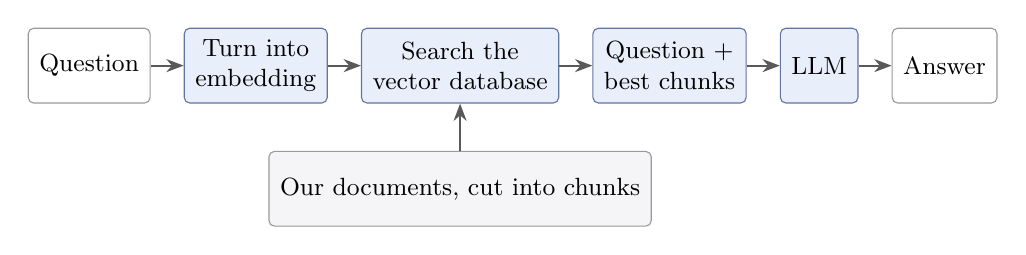
\begin{tikzpicture}[node distance=0.45cm and 0.42cm]
  \node[plain] (q) {Question};
  \node[blk, right=of q] (e) {Turn into\\embedding};
  \node[blk, right=of e] (s) {Search the\\vector database};
  \node[blk, right=of s] (p) {Question +\\best chunks};
  \node[blk, right=of p] (l) {LLM};
  \node[plain, right=of l] (a) {Answer};
  \node[plain, below=0.6cm of s, fill=softgrey] (d) {Our documents, cut into chunks};
  \draw[arr] (q)--(e); \draw[arr] (e)--(s); \draw[arr] (s)--(p);
  \draw[arr] (p)--(l); \draw[arr] (l)--(a); \draw[arr] (d)--(s);
\end{tikzpicture}}
\caption{How RAG works, in short}\label{fig:rag}
\end{figure}

The later days covered \emph{evaluating} RAG (check that search finds the right chunks
before blaming the model) and advanced ideas like reranking and query rewriting. I used the
evaluation habit directly when choosing how strict my search should be
(Section~\ref{sec:threshold}).

\section{Weeks 6 and 7: Fine-Tuning}
\emph{Fine-tuning} means training an existing model a little more on examples of one task.
Weeks 6 and 7 were one project that predicts a product's price from its description. Before
any LLM, we cleaned the data and built simple baselines (random forest, XGBoost, a small
neural network), then fine-tuned a frontier model with examples in JSONL format. Week 7 used
\emph{LoRA}, which keeps the model frozen and trains only small extra matrices, and
\emph{QLoRA}, which also stores the frozen model in 4 bits so that an 8-billion-parameter
model can be trained on one free Colab GPU. The main lesson: RAG gives a model new
\emph{knowledge}, while fine-tuning changes its \emph{behaviour}. That is why StudyPilot uses
RAG for the student's notes.

\section{Week 8: Agents}
An \emph{agent} is a loop (Figure~\ref{fig:agent}): the model gets a list of tools, decides
whether it needs one, our code runs it and sends back the result, and this repeats until the
model can answer. The capstone combined everything: agents that scanned deal websites,
estimated prices (including the fine-tuned model running on Modal and RAG over 400,000
products), sent phone notifications, and a planner that decided which to call. StudyPilot
does not need a full agent loop, because its steps always happen in the same order, but it
uses the same idea of chaining model calls with code checks in between.

\begin{figure}[H]
\centering
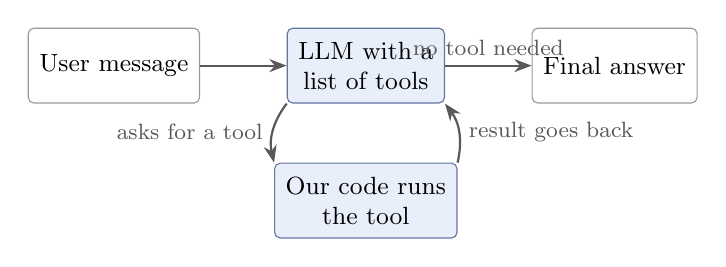
\begin{tikzpicture}[node distance=0.5cm and 1.1cm]
  \node[plain] (u) {User message};
  \node[blk, right=of u] (m) {LLM with a\\list of tools};
  \node[plain, right=of m] (f) {Final answer};
  \node[blk, below=0.75cm of m] (t) {Our code runs\\the tool};
  \draw[arr] (u)--(m);
  \draw[arr] (m)--node[above,font=\footnotesize]{no tool needed}(f);
  \draw[arr] (m.south west) to[bend right=25] node[left,font=\footnotesize]{asks for a tool} (t.north west);
  \draw[arr] (t.north east) to[bend right=25] node[right,font=\footnotesize]{result goes back} (m.south east);
\end{tikzpicture}
\caption{The agent loop}\label{fig:agent}
\end{figure}

\section{From the Course to my Project}
Table~\ref{tab:courseuse} shows where each idea from the course shows up in StudyPilot. The
biggest takeaways for me were: give the model the facts (RAG), remember that the model
forgets everything, and measure a change before trusting it.

\begin{table}[H]
\centering
\caption{Course ideas used in the project}\label{tab:courseuse}
\small
\begin{tabularx}{\textwidth}{@{}P{4.2cm}L@{}}
\toprule
\textbf{Course idea (week)} & \textbf{Where it is used in StudyPilot} \\
\midrule
OpenAI-compatible APIs (1)     & One \code{openai} package talks to Ollama and to Gemini \\
System prompts (1, 2)          & Separate prompts for answering from notes and for general chat \\
Stateless calls, memory (1, 2) & The last six messages are sent again with every question \\
Streaming, JSON output (1)     & Chat answers stream word by word; cards and quizzes come back as JSON \\
Quantisation, model choice (3, 4) & A 4-bit Qwen2.5 1.5B model fits fully in my 4\,GB GPU \\
Embeddings, Chroma, RAG (5)    & The whole library is chunked, embedded and searched with Chroma \\
Evaluating retrieval (5)       & Search scores were measured before choosing a relevance cut-off \\
JSONL data, fine-tuning (6, 7) & A small JSONL dataset for grading short answers (future work) \\
\bottomrule
\end{tabularx}
\end{table}

% =====================================================================
\chapter{Project Design}
% =====================================================================

\section{Main Features}
StudyPilot is a web app for students who want to study from their own material. It has
four main parts:
\begin{enumerate}
  \item \textbf{Library.} Upload PDFs, scanned pages or photos, or paste a YouTube link.
        Everything becomes searchable text.
  \item \textbf{Chat.} Answers come from the library, with the file and page shown as
        coloured ``citation chips''. Small talk and general questions get a normal answer,
        marked as not coming from the library.
  \item \textbf{Flashcards.} Decks on any topic in the library, which come back after 1, 2,
        4, 8 or 16 days depending on how well each card is known.
  \item \textbf{Quiz.} Multiple-choice and short-answer questions with a score, feedback on
        every answer, and a button that turns missed questions into a deck.
\end{enumerate}

\section{Architecture}
Figure~\ref{fig:arch} shows how the parts fit together. The React frontend talks only to my
FastAPI backend through a REST API that sends JSON. The backend has an \emph{indexer} that
reads files and videos into chunks, a \emph{RAG} part that searches them, a \emph{chat} part
that streams answers from the local model, and \emph{flashcards} and \emph{quiz} parts that
call Gemini. The original files are kept in a folder, the chunks and embeddings in ChromaDB,
and the flashcards, quizzes and progress in SQLite. The notes go to the cloud only when the
student makes flashcards or a quiz; chat stays on the laptop. Table~\ref{tab:stack} lists the
tools.

\begin{figure}[H]
\centering
\resizebox{\textwidth}{!}{%
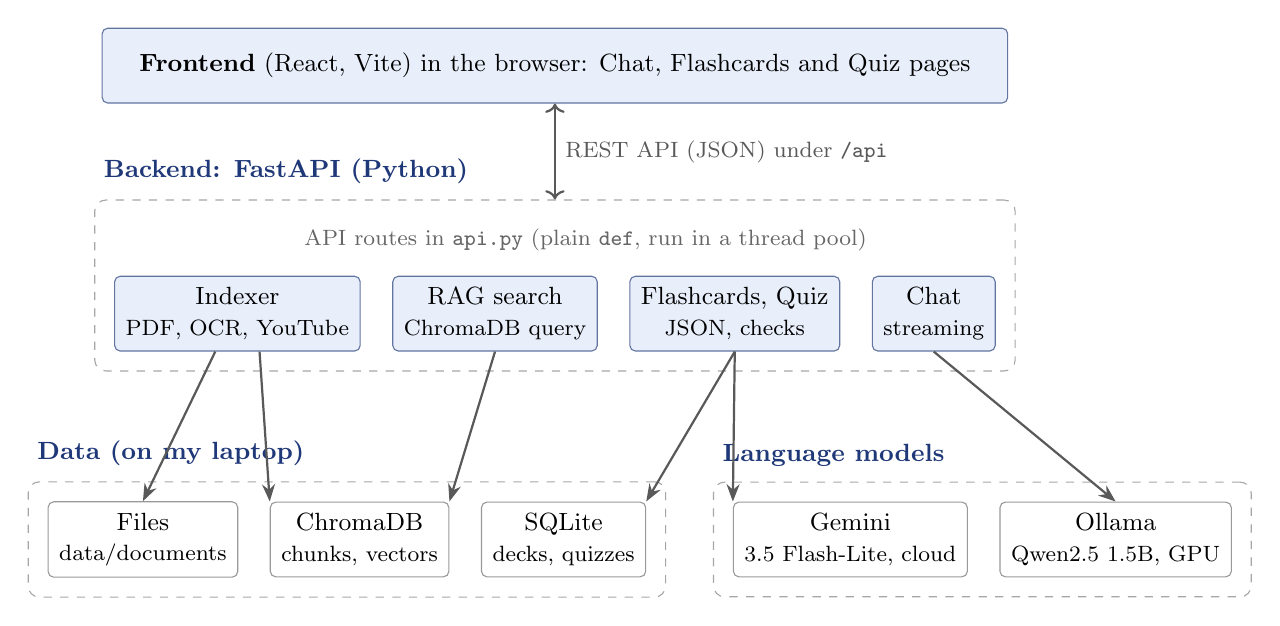
\begin{tikzpicture}[node distance=0.4cm]
  % backend modules, placed one after another
  \node[blk] (ix) {Indexer\\{\footnotesize PDF, OCR, YouTube}};
  \node[blk, right=of ix] (rg) {RAG search\\{\footnotesize ChromaDB query}};
  \node[blk, right=of rg] (fq) {Flashcards, Quiz\\{\footnotesize JSON, checks}};
  \node[blk, right=of fq] (ch) {Chat\\{\footnotesize streaming}};
  \node[font=\footnotesize, text=black!60] (rt) at ($(ix.north)!0.5!(ch.north)+(0,0.45)$)
       {API routes in \code{api.py} (plain \code{def}, run in a thread pool)};
  \node[grp, fit=(rt)(ix)(rg)(fq)(ch)] (be) {};
  \node[grplabel] at ([yshift=2pt]be.north west) {Backend: FastAPI (Python)};
  % browser on top
  \node[blk, minimum width=11.5cm] (fe) at ([yshift=1.7cm]be.north)
       {\textbf{Frontend} (React, Vite) in the browser: Chat, Flashcards and Quiz pages};
  \draw[arr,<->] (fe.south) -- node[right,font=\footnotesize]{REST API (JSON) under \code{/api}} (be.north);
  % data and models underneath
  \node[plain, anchor=north] (fs) at ([xshift=-1.2cm,yshift=-1.9cm]ix.south) {Files\\{\footnotesize data/documents}};
  \node[plain, right=of fs] (cd) {ChromaDB\\{\footnotesize chunks, vectors}};
  \node[plain, right=of cd] (sq) {SQLite\\{\footnotesize decks, quizzes}};
  \node[grp, fit=(fs)(cd)(sq)] (data) {};
  \node[grplabel] at ([yshift=2pt]data.north west) {Data (on my laptop)};
  \node[plain, right=1.1cm of sq] (gm) {Gemini\\{\footnotesize 3.5 Flash-Lite, cloud}};
  \node[plain, right=of gm] (ol) {Ollama\\{\footnotesize Qwen2.5 1.5B, GPU}};
  \node[grp, fit=(gm)(ol)] (mods) {};
  \node[grplabel] at ([yshift=2pt]mods.north west) {Language models};
  % arrows, ordered left to right so none of them cross
  \draw[arr] ([xshift=-8pt]ix.south) -- (fs.north);
  \draw[arr] ([xshift=8pt]ix.south) -- (cd.north west);
  \draw[arr] (rg.south) -- (cd.north east);
  \draw[arr] (fq.south) -- (sq.north east);
  \draw[arr] (fq.south) -- (gm.north west);
  \draw[arr] (ch.south) -- (ol.north);
\end{tikzpicture}}
\caption{Architecture of StudyPilot}\label{fig:arch}
\end{figure}

\begin{table}[H]
\centering
\caption{Technology stack}\label{tab:stack}
\small
\begin{tabularx}{\textwidth}{@{}P{2.6cm}P{4.6cm}L@{}}
\toprule
\textbf{Part} & \textbf{Tool} & \textbf{Why} \\
\midrule
Backend        & Python, FastAPI            & Quick to write; checks request data; free test page \\
Frontend       & React, Vite                & Pages from small reusable parts; fast reloads \\
Chat model     & Qwen2.5 1.5B on Ollama     & Free, private, fits fully in a 4\,GB GPU \\
Study model    & Gemini 3.5 Flash-Lite      & Free tier; reliable JSON for cards, questions, grades \\
Search         & ChromaDB, all-MiniLM-L6-v2 & Runs locally; the same tools as in the course \\
Database       & SQLite                     & One file, built into Python \\
Reading input  & PyMuPDF, EasyOCR, youtube-transcript-api & PDF text, scans and photos, transcripts \\
\bottomrule
\end{tabularx}
\end{table}

\section{API Design}
\begin{wrapfigure}{r}{0.36\textwidth}
\vspace{-14pt}
\centering
\fcolorbox{black!25}{white}{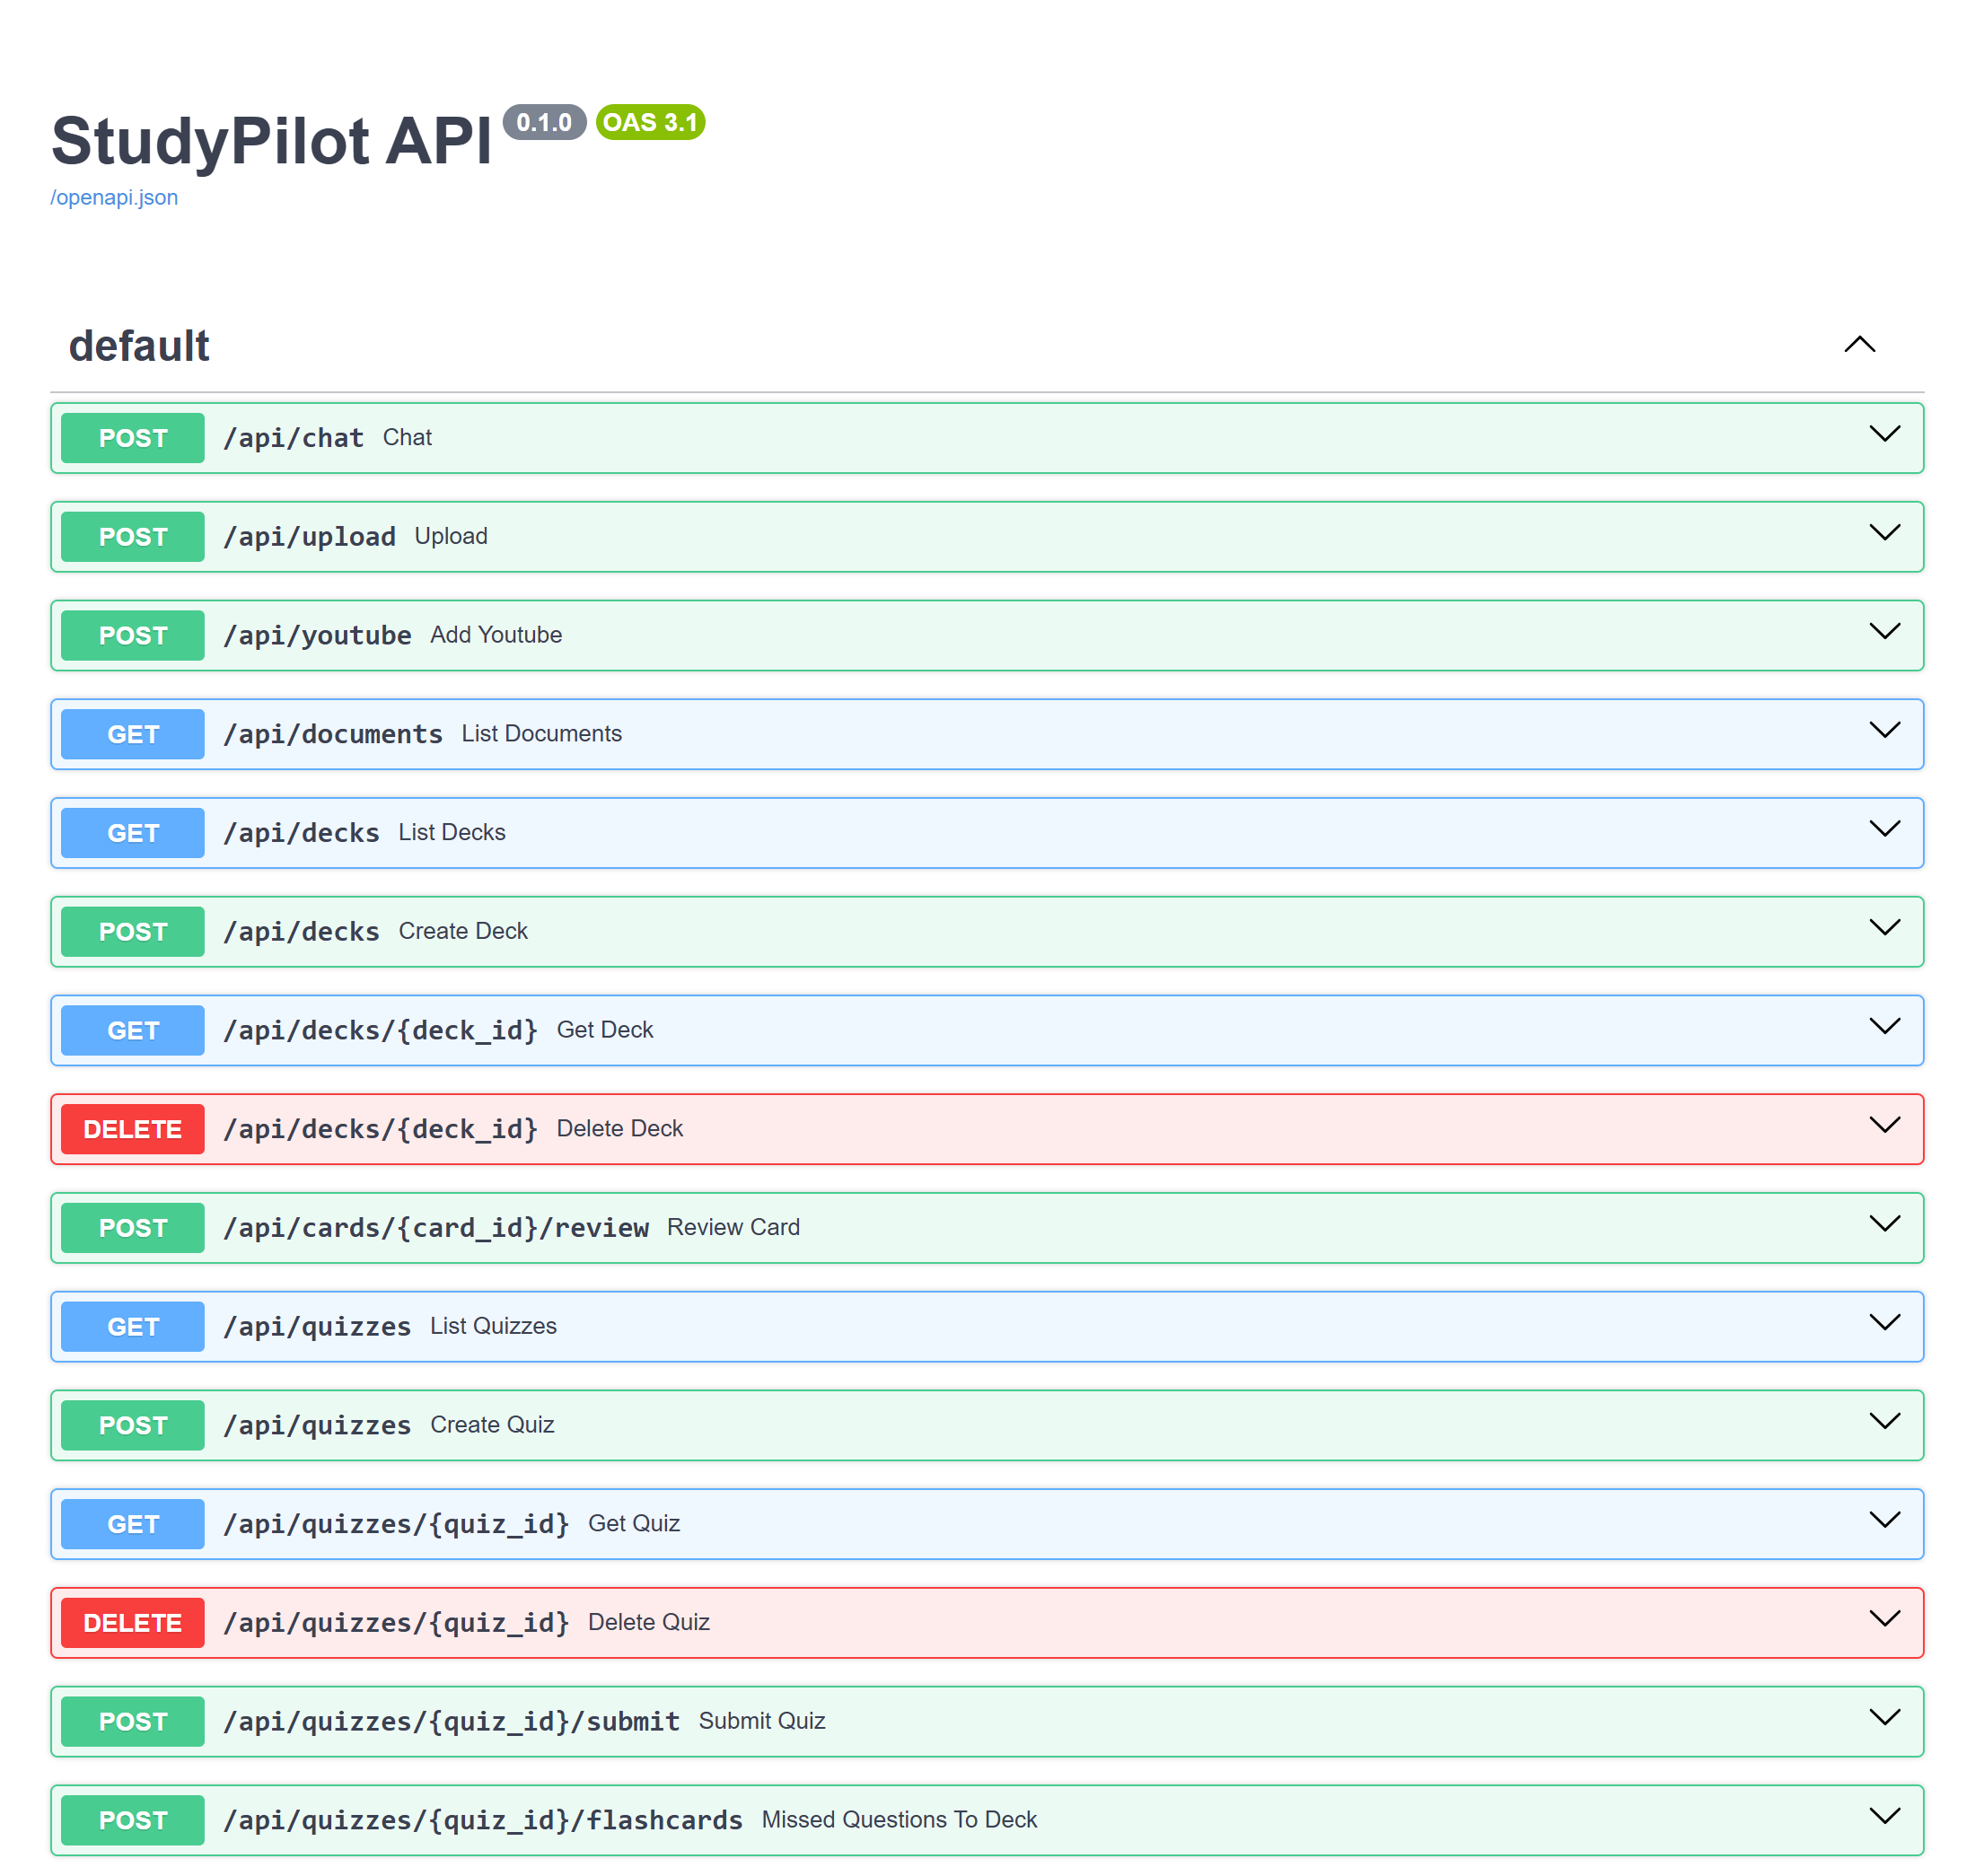
\includegraphics[width=0.33\textwidth]{fastapi-docs.png}}
\caption{FastAPI's automatic test page}\label{fig:docs}
\vspace{-12pt}
\end{wrapfigure}
The backend is a REST API: the frontend sends a request to a URL with a method (GET to read,
POST to create or run an action, DELETE to remove) and gets JSON back. Table~\ref{tab:api}
groups the routes, and Figure~\ref{fig:docs} shows the test page FastAPI builds on its own at
\code{/docs}, which I used a lot before the frontend was ready. During development, the Vite
server forwards every \code{/api} request to the backend, so no cross-origin setup is needed.

All routes use plain \code{def}, not \code{async def}. OCR, embeddings and LLM calls are slow,
and FastAPI runs plain \code{def} routes in a pool of threads, so a slow upload does not
freeze the chat. I tested this by uploading a scanned PDF while asking a question; neither
waited for the other.

\begin{table}[H]
\centering
\caption{Main API routes}\label{tab:api}
\small
\begin{tabularx}{\textwidth}{@{}P{2.0cm}P{7.3cm}L@{}}
\toprule
\textbf{Group} & \textbf{Routes} & \textbf{What they do} \\
\midrule
Library    & POST \code{/api/upload}, POST \code{/api/youtube}, GET \code{/api/documents} & Add material; list it \\
Chat       & POST \code{/api/chat} & Answer a question (streamed) \\
Flashcards & GET, POST \code{/api/decks}; GET, DELETE \code{/api/decks/\{id\}}; POST \code{/api/cards/\{id\}/review} & Decks and reviews \\
Quiz       & GET, POST \code{/api/quizzes}; GET, DELETE \code{/api/quizzes/\{id\}}; POST \code{.../submit}, \code{.../flashcards} & Quizzes, grading, missed questions \\
\bottomrule
\end{tabularx}
\end{table}

% =====================================================================
\chapter{How the Project Works}
% =====================================================================

\section{Adding Study Material}
Every input is turned into the same shape: a list of ``pages'', each with a source name, a
page number and its text (Figure~\ref{fig:index}). PDFs are read page by page with PyMuPDF.
If a page gives fewer than 50 characters, it is treated as scanned: it is turned into an
image at 200 DPI and read with EasyOCR. Photos are read the same way. On a test scan, the OCR
text matched 94\% of the words of the original. YouTube lectures are read from their
transcripts, grouped into 5-minute sections that act like pages; my sharding lecture became
17 sections.

\begin{figure}[H]
\centering
\resizebox{\textwidth}{!}{%
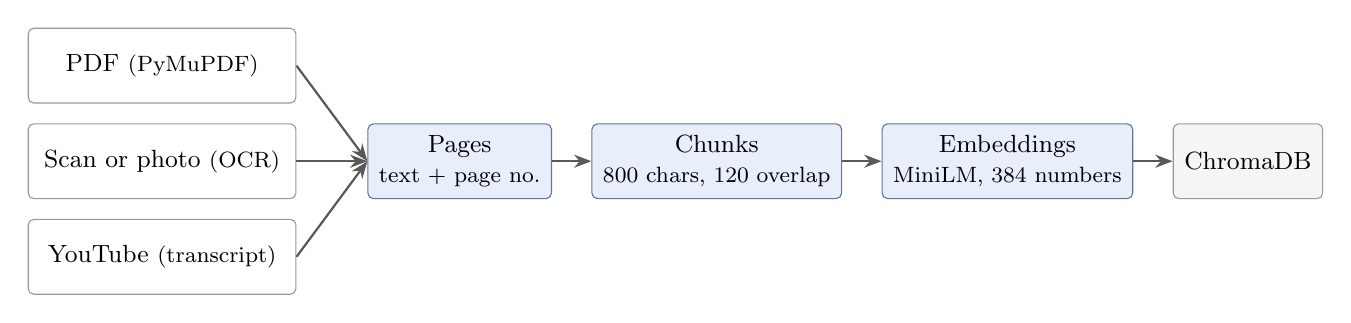
\begin{tikzpicture}[node distance=0.25cm and 0.5cm]
  \node[plain, minimum width=3.4cm] (img) {Scan or photo {\footnotesize (OCR)}};
  \node[plain, minimum width=3.4cm, above=of img] (pdf) {PDF {\footnotesize (PyMuPDF)}};
  \node[plain, minimum width=3.4cm, below=of img] (yt) {YouTube {\footnotesize (transcript)}};
  \node[blk, right=0.9cm of img] (pg) {Pages\\{\footnotesize text + page no.}};
  \node[blk, right=of pg] (ck) {Chunks\\{\footnotesize 800 chars, 120 overlap}};
  \node[blk, right=of ck] (em) {Embeddings\\{\footnotesize MiniLM, 384 numbers}};
  \node[plain, fill=softgrey, right=of em] (db) {ChromaDB};
  \draw[arr] (pdf.east) -- (pg.west);
  \draw[arr] (img.east) -- (pg.west);
  \draw[arr] (yt.east)  -- (pg.west);
  \draw[arr] (pg)--(ck); \draw[arr] (ck)--(em); \draw[arr] (em)--(db);
\end{tikzpicture}}
\caption{Steps for adding study material to the library}\label{fig:index}
\end{figure}

The pages are cut into chunks of 800 characters with 120 characters of overlap, so a
sentence cut at an edge still appears whole in one chunk. Each chunk is embedded and stored
in ChromaDB with its source and page. Uploading the same file again first deletes its old
chunks. My test library (two computer-architecture lecture PDFs, a PDF on consistent hashing
and a YouTube lecture on database sharding) made 162 chunks.

\section{Answering a Question}\label{sec:chat}
The question is embedded and ChromaDB returns the four closest chunks, each with a
\emph{cosine distance} (0 means the same meaning). Chunks with a distance above
\textbf{0.65} are dropped; this number was measured (Section~\ref{sec:threshold}). Then:
\begin{itemize}
  \item \textbf{Study mode.} The chunks go into the prompt, each labelled with its source
        (for example \code{[class16.pdf, page 12]}), and the model must answer from them
        and cite those labels. The browser turns each label into a pink citation chip.
  \item \textbf{General mode.} If no chunk is close enough (``how are you?'', ``capital of
        France?''), another system prompt lets the model reply from its own knowledge, and
        the answer is marked ``General answer \textperiodcentered{} not from your library''.
\end{itemize}
My first version always used the four closest chunks, so ``how are you'' got an answer about
database sharding. The cut-off and the two modes fixed this.

Answers are \textbf{streamed}: while the model writes, the backend sends one small JSON object
per line (first the sources, then pieces of text, then ``done''), and the browser adds each
piece as it arrives. For \textbf{memory}, the browser sends the last six messages with every
question, and earlier answers carry a note of their sources so that follow-ups like ``is this
from my PDF?'' are answered correctly. Small prompt details mattered too: when the excerpts
were numbered ``Passage 1, 2'', the model wrote ``Passage 2 says\ldots'' in its answers, and
a made-up example label in the prompt was once copied as a fake citation. Now the excerpts
carry only real source labels.

\begin{figure}[H]
\centering
\fcolorbox{black!25}{white}{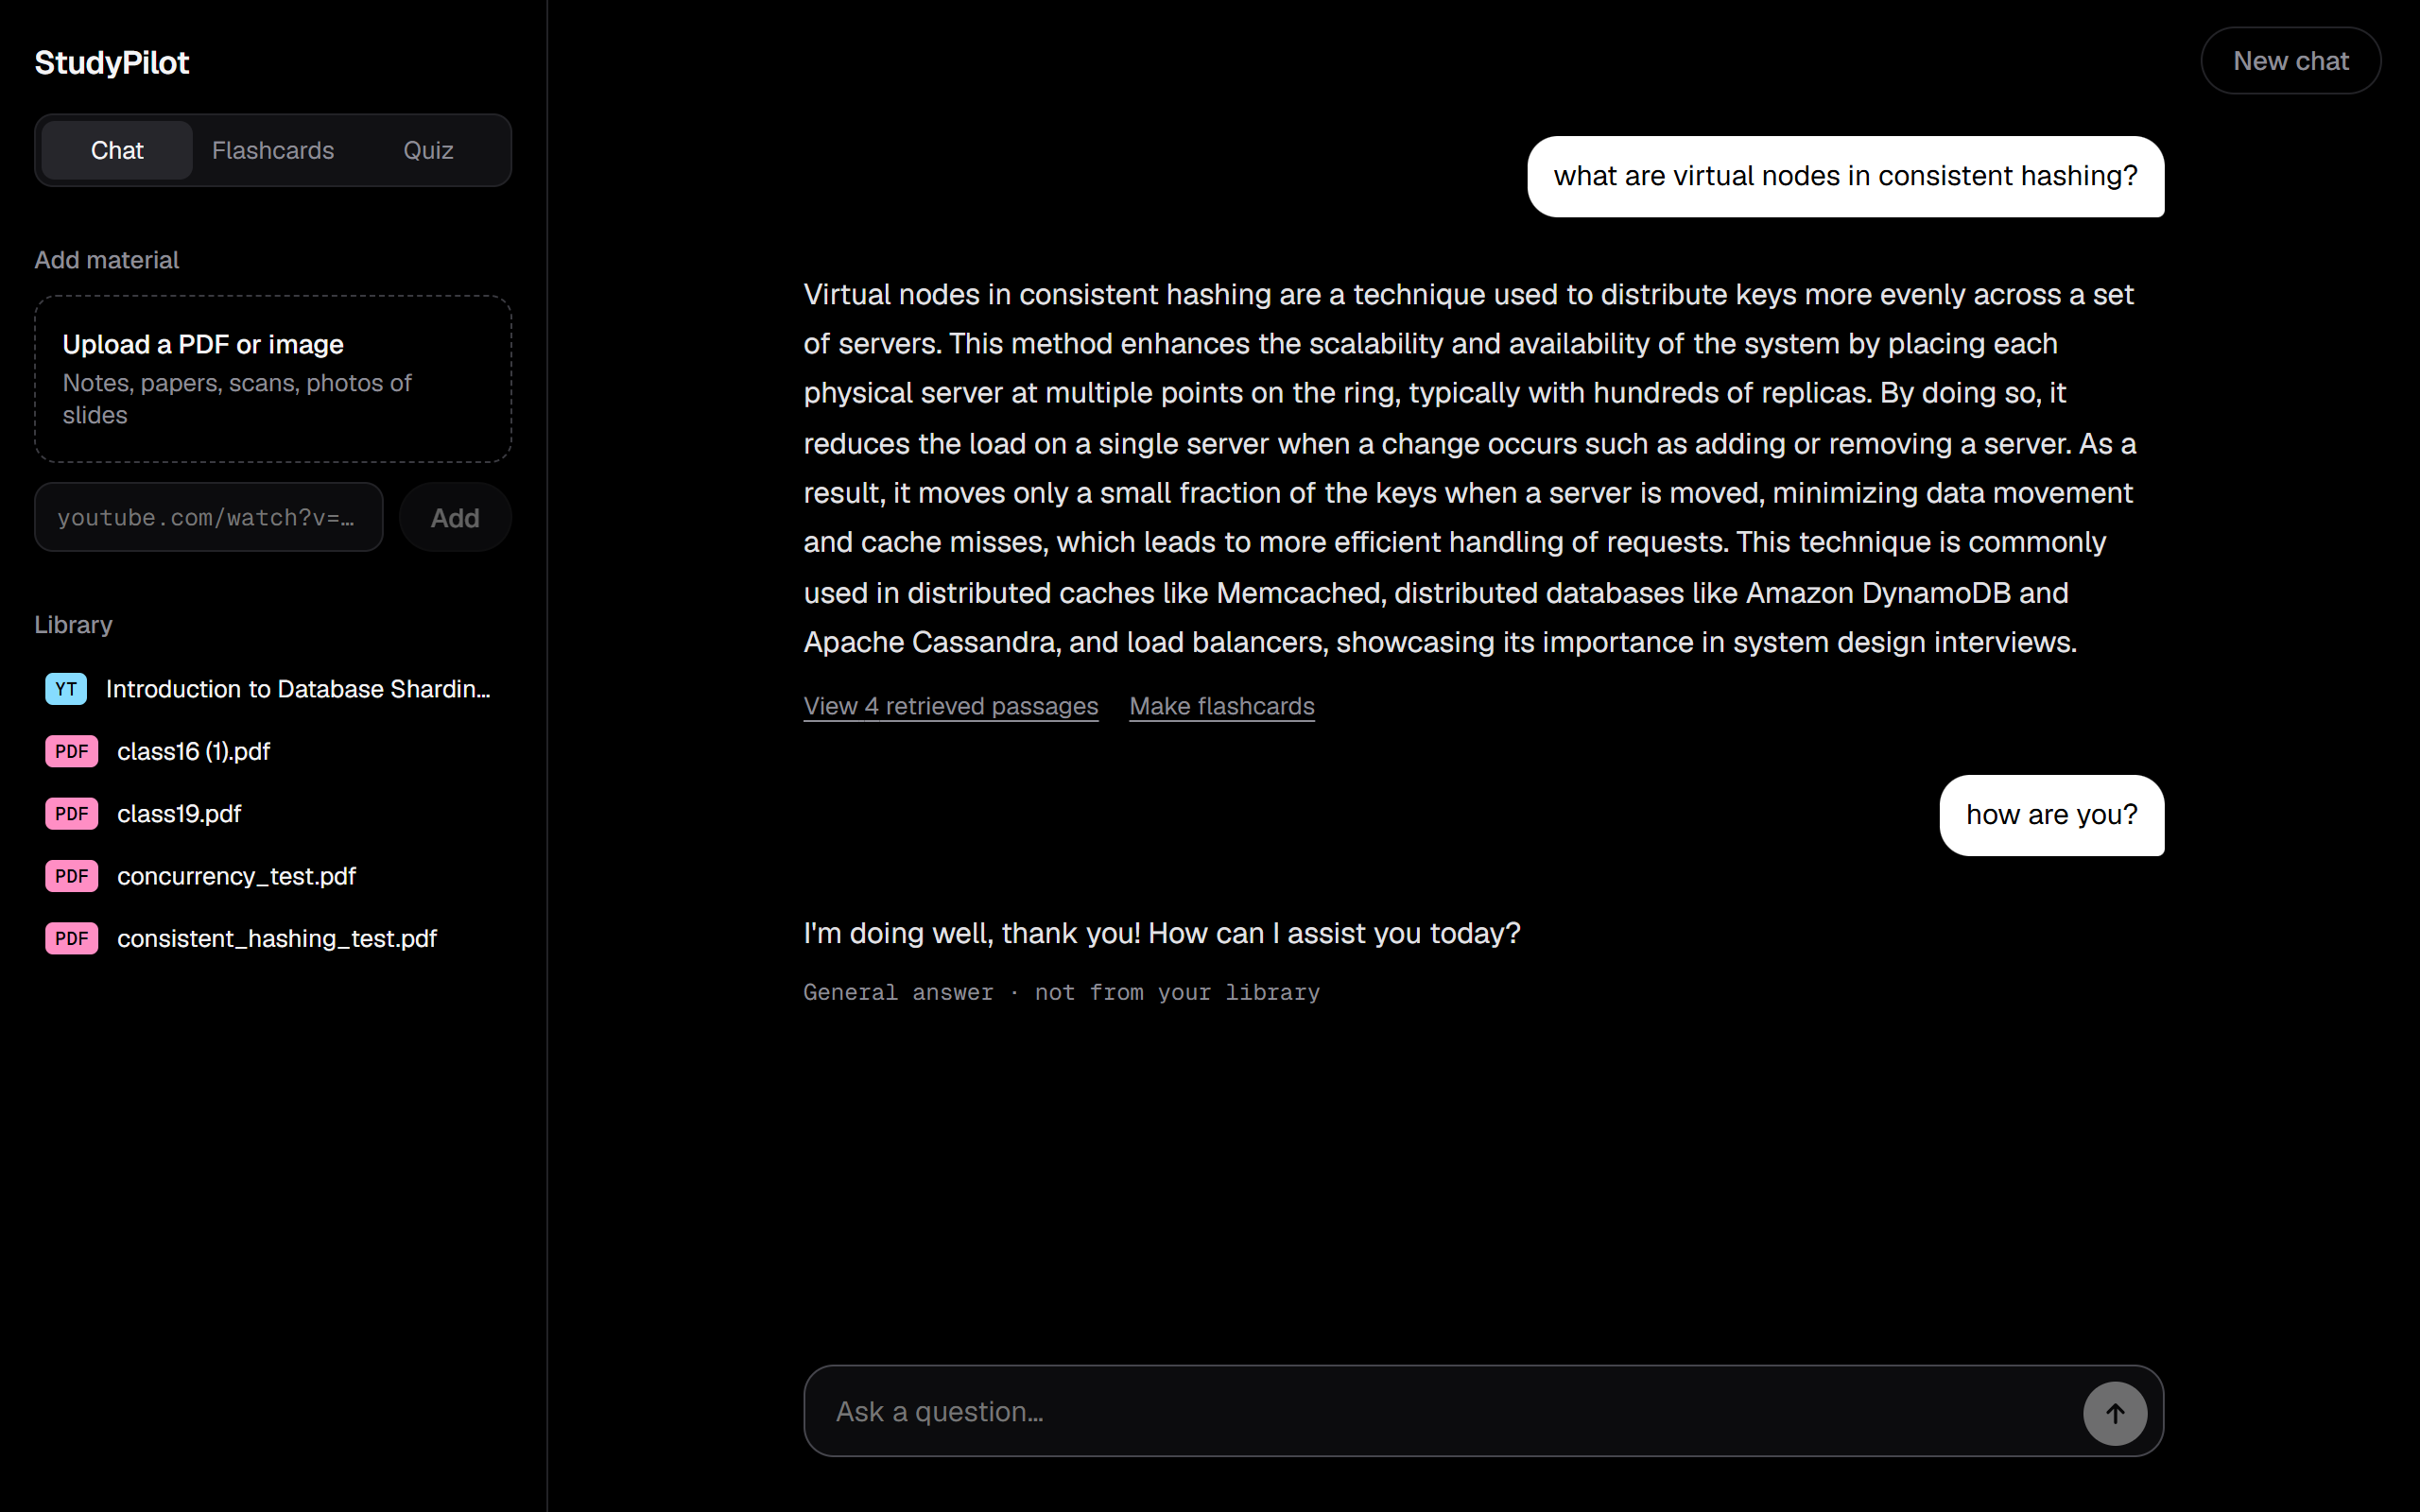
\includegraphics[width=0.8\textwidth]{chat.png}}
\caption{Chat: an answer from the library, then a general answer}\label{fig:chat}
\end{figure}

\section{Flashcards with Spaced Repetition}
For a deck, the student types a topic and picks 5 to 20 cards. The backend retrieves eight
chunks on the topic and sends them to Gemini with a JSON schema (front, back, source, page),
which forces a reply in exactly that shape. Python keeps only complete cards and removes any
source that was not one of the chunks sent, so the model cannot invent a page. Revision uses
the \emph{Leitner system} \cite{leitner} (Figure~\ref{fig:leitner}): ``Got it'' moves a card
up one box and ``Again'' sends it back to box 1, and higher boxes come back less often.
A card marked ``Again'' also goes to the back of the current session.

\begin{figure}[H]
\centering
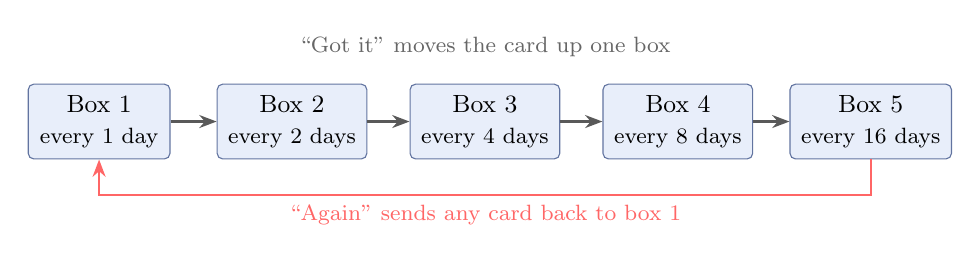
\begin{tikzpicture}[node distance=0.55cm]
  \foreach \i/\d in {1/1,2/2,3/4,4/8,5/16} {
    \node[blk, minimum width=1.8cm] (b\i) at ({(\i-1)*2.45},0) {Box \i\\{\footnotesize every \d\ day\ifnum\d>1 s\fi}};
  }
  \foreach \i/\j in {1/2,2/3,3/4,4/5} { \draw[arr] (b\i) -- (b\j); }
  \node[font=\footnotesize, text=black!60] at (4.9,0.95) {``Got it'' moves the card up one box};
  \draw[arr, draw=red!60] (b5.south) -- ++(0,-0.45) -| node[pos=0.25,below,font=\footnotesize,text=red!60]{``Again'' sends any card back to box 1} (b1.south);
\end{tikzpicture}
\caption{The Leitner boxes used for flashcards}\label{fig:leitner}
\end{figure}

\begin{figure}[H]
\centering
\begin{subfigure}{0.49\textwidth}\centering
  \fcolorbox{black!25}{white}{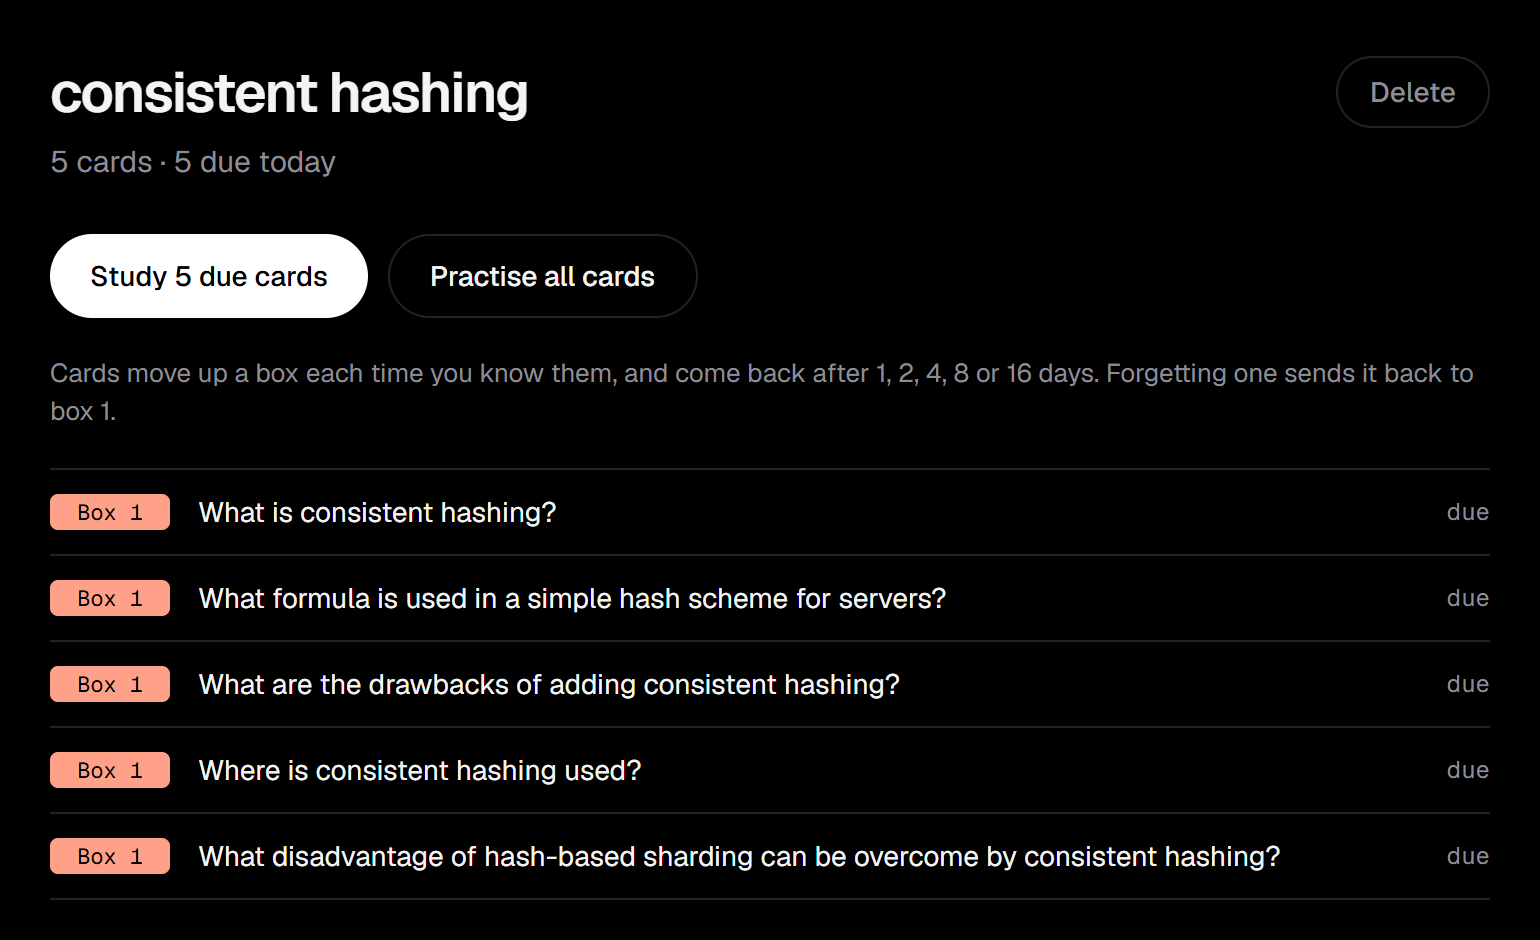
\includegraphics[width=0.95\linewidth]{deck.png}}
  \caption{A deck with box numbers}
\end{subfigure}\hfill
\begin{subfigure}{0.49\textwidth}\centering
  \fcolorbox{black!25}{white}{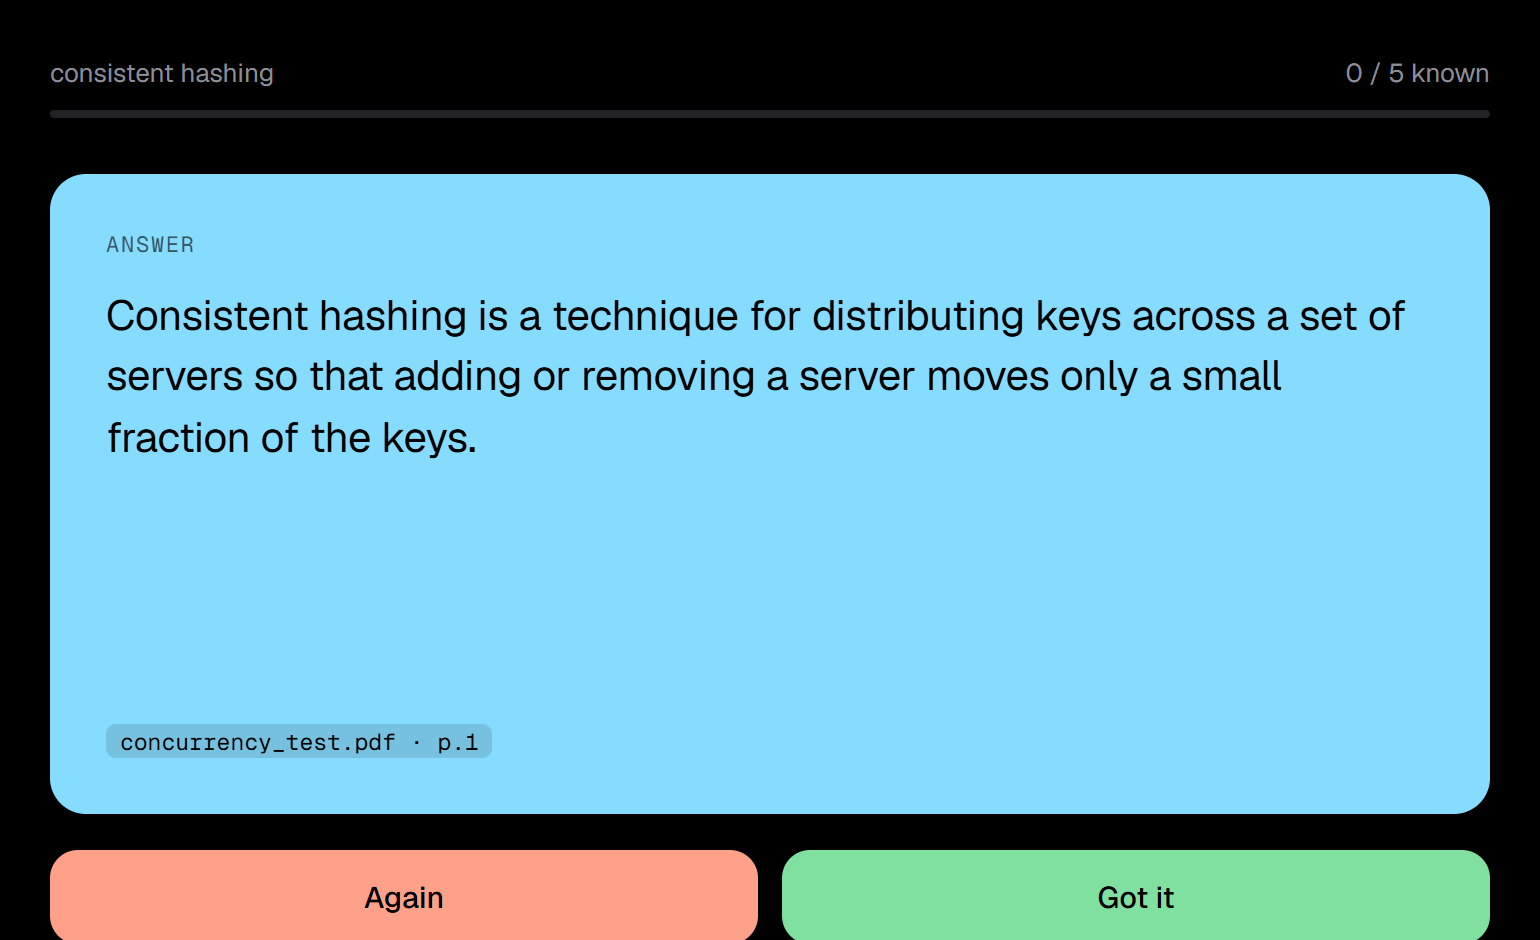
\includegraphics[width=0.95\linewidth]{flashcard-back.png}}
  \caption{A card turned over, with its source}
\end{subfigure}
\caption{Flashcards}\label{fig:flashcards}
\end{figure}

\section{Quiz and Grading}
A quiz is made the same way: a topic, 5 to 15 questions, and multiple-choice, short-answer or
mixed. Python checks that every multiple-choice question has four options and a valid answer,
and shuffles the options because LLMs often put the right one first. The answers stay on the
server until the quiz is submitted. \textbf{Multiple choice} is graded by plain Python, which
is instant and always correct. \textbf{Short answers} are graded by Gemini in one request:
for each it returns a score from 0 to 5, the key points the student got right, the missing
points, short feedback and a next step (Figure~\ref{fig:quiz}b). This is the same format as
my small training dataset for a future fine-tuned grader. Questions that earned less than
60\% can be turned into a flashcard deck with one click, without any LLM call.

\begin{figure}[H]
\centering
\begin{subfigure}{0.49\textwidth}\centering
  \fcolorbox{black!25}{white}{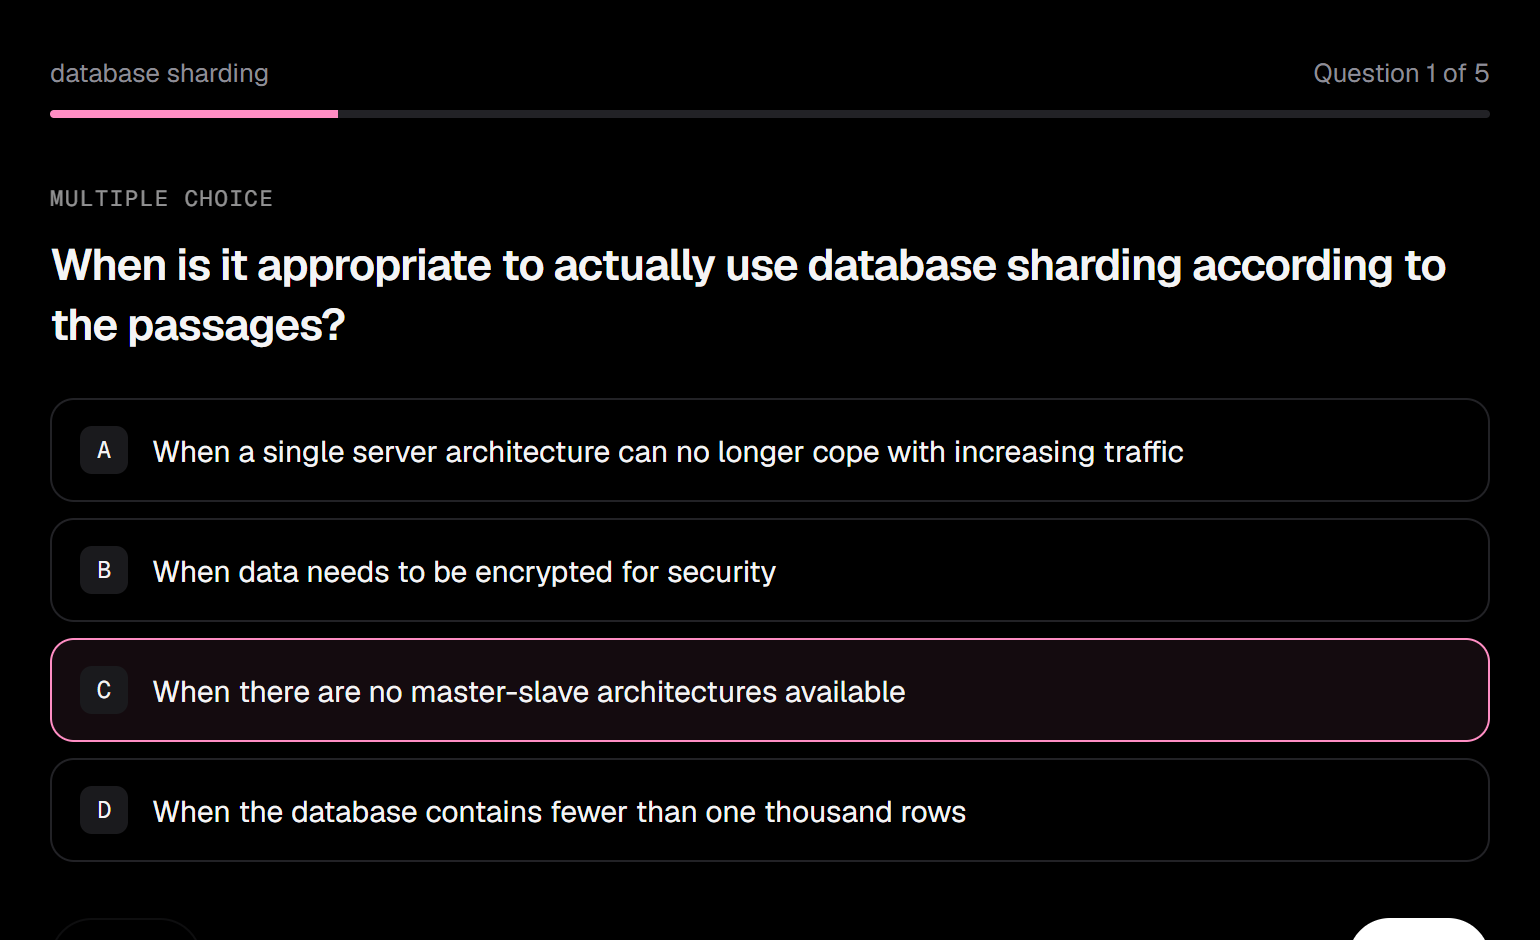
\includegraphics[width=0.95\linewidth]{quiz-question.png}}
  \caption{A multiple-choice question}
\end{subfigure}\hfill
\begin{subfigure}{0.49\textwidth}\centering
  \fcolorbox{black!25}{white}{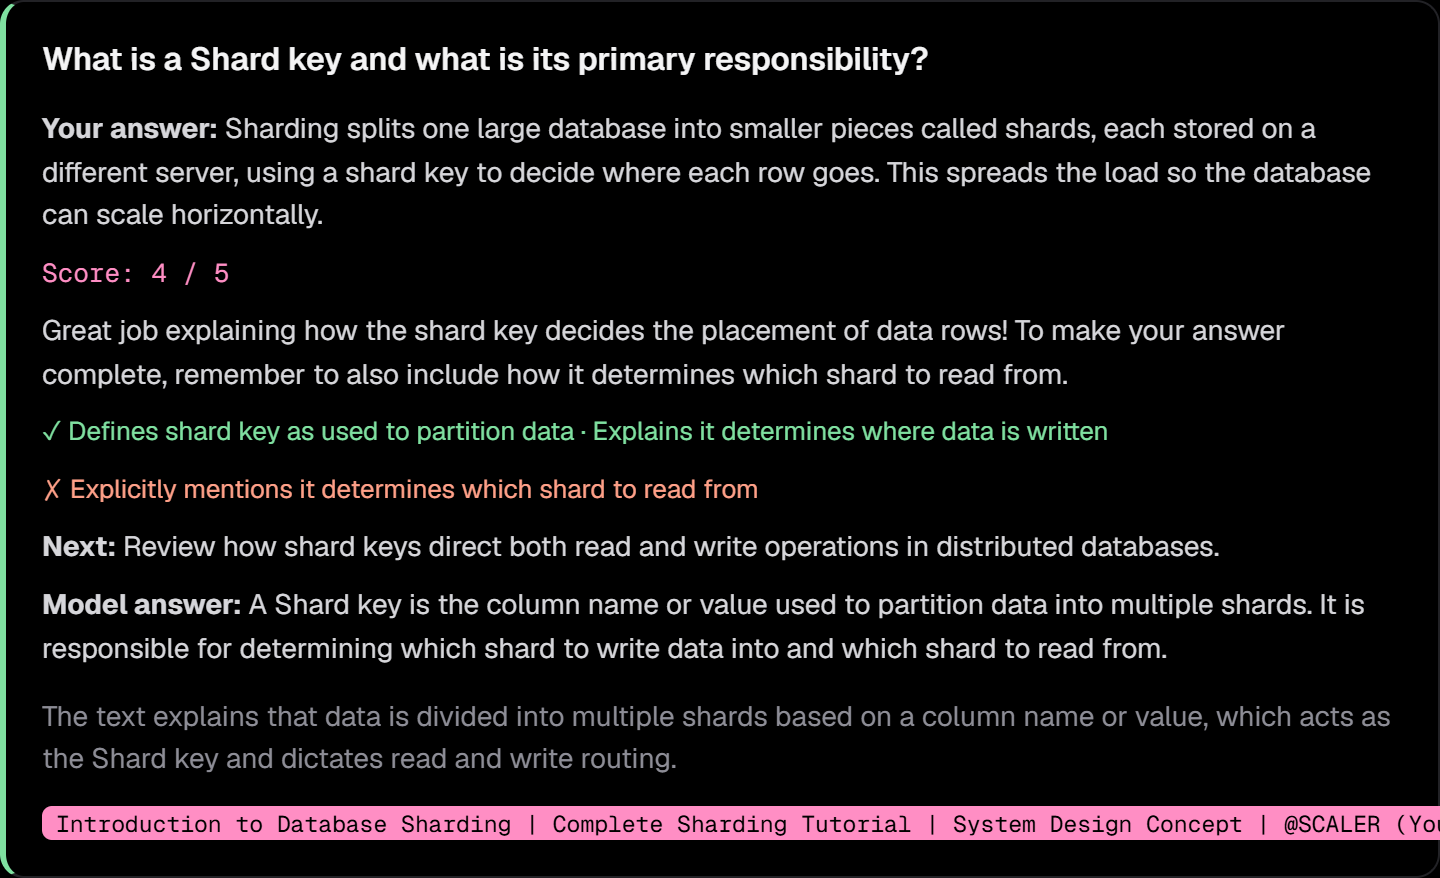
\includegraphics[width=0.95\linewidth]{quiz-short-feedback.png}}
  \caption{Feedback on a short answer}
\end{subfigure}
\caption{Taking a quiz and getting feedback}\label{fig:quiz}
\end{figure}

% =====================================================================
\chapter{Testing and Results}
% =====================================================================

\section{Choosing the Relevance Cut-off}\label{sec:threshold}
Following the week 5 lesson on evaluating retrieval, I did not guess the cut-off. I asked
nine questions about my notes and ten general questions, and noted the distance of the best
chunk for each (Table~\ref{tab:threshold}). Questions about the notes scored 0.13 to 0.61 and
general questions scored 0.69 to 0.86, so a cut-off of 0.65 separates them.

\begin{table}[H]
\centering
\caption{Distance of the best chunk for some test questions}\label{tab:threshold}
\small
\begin{tabular}{@{}lc@{\hspace{1.4cm}}lc@{}}
\toprule
\textbf{About my notes} & \textbf{Distance} & \textbf{General} & \textbf{Distance} \\
\midrule
What is consistent hashing?           & 0.13 & Explain recursion                & 0.69 \\
Instruction level parallelism         & 0.27 & What is photosynthesis?          & 0.77 \\
How does database sharding work?      & 0.31 & hi                               & 0.79 \\
What is MIMD?                         & 0.57 & how are you                      & 0.85 \\
Explain Flynn's taxonomy              & 0.61 & Capital of France?               & 0.86 \\
\bottomrule
\end{tabular}
\end{table}

\section{Test Cases and Speed}
I tested the API with curl and Python scripts, and the screens with a browser-automation
script in Chrome. All the cases in Table~\ref{tab:tests} passed. On my laptop, the sources of
an answer appear in about 0.1\,s, the first words in about 2.5\,s, and a full answer in 3 to
10\,s. Making a deck takes about 3\,s, a quiz about 4\,s, and grading about 2\,s.

\begin{table}[H]
\centering
\caption{Test cases}\label{tab:tests}
\small
\begin{tabularx}{\textwidth}{@{}cP{5.4cm}Lc@{}}
\toprule
\textbf{No.} & \textbf{Test} & \textbf{Result} & \textbf{Status} \\
\midrule
1  & Upload a \code{.txt} file                & Error 400 with the allowed types & Pass \\
2  & Upload a scanned PDF and a photo         & OCR used; 94\% of words matched & Pass \\
3  & Add a non-YouTube link                   & Error 400 with a clear message & Pass \\
4  & Upload and chat at the same time         & Both finished, neither waited & Pass \\
5  & Ask ``how are you''                      & Friendly reply, marked general & Pass \\
6  & ``Is this from my PDF?'' after a cited answer & ``Yes'', with the right file & Pass \\
7  & Chat while the model is unavailable      & Error message shown in the chat & Pass \\
8  & Open a quiz before submitting            & No correct answers sent & Pass \\
9  & Submit the same quiz twice               & Error 400, ``already submitted'' & Pass \\
10 & ``Got it'' twice, then ``Again''         & Box 1 $\rightarrow$ 2 $\rightarrow$ 3 $\rightarrow$ 1 & Pass \\
\bottomrule
\end{tabularx}
\end{table}

\section{Problems Found and Fixed}
The strangest problem was that Gemini requests often failed with an SSL ``bad record mac''
error and took 10 to 28 seconds when they worked. Testing step by step showed that my
network's IPv6 connection to Google was the cause: over IPv6, 0 of 5 large requests worked,
while over IPv4, 5 of 5 worked in about 1.5 seconds. The Gemini client now always uses IPv4.
Other fixes included freeing GPU memory after OCR, turning off a progress bar that crashed
the OCR model download on Windows, and using the local date (not UTC) for ``due today''.

% =====================================================================
\chapter{Conclusion and Future Scope}
% =====================================================================

\section{What I Learnt}
Before this internship I thought building with AI meant writing one clever prompt. I now see
it as normal software engineering with one unreliable part in the middle. The model is good
at reading and writing, but not at following every rule or knowing where its knowledge came
from. So the real work is deciding what the model should do and what plain code should do,
giving it the right text (RAG), and checking what comes back. I also learnt to measure
instead of guessing: the model, the cut-off and the OCR settings were all chosen by testing.

\section{Limitations}
\begin{itemize}
  \item The small 1.5B model does not always cite its sources: 5 of 12 test answers had
        proper citations. The passages used are always listed, though.
  \item The 0.65 cut-off was measured on my notes; very different subjects may need it
        measured again. Follow-ups like ``tell me more about them'' search only the newest
        question.
  \item There is no login and no way to delete a document yet, so it suits one student on
        one computer.
  \item Flashcards and quizzes depend on Gemini's free tier, which has daily limits.
\end{itemize}

\section{Conclusion and Future Scope}
The course gave me a clear, hands-on base in LLM engineering, from API calls to RAG,
fine-tuning and agents. StudyPilot puts most of these ideas into one working app: it reads
PDFs, scanned notes and YouTube lectures into one library, answers from them with citations,
knows when a question is not about the notes, and helps revision with spaced-repetition
flashcards and graded quizzes, while chat runs fully on a 4\,GB laptop GPU. In future, I want
to fine-tune a small model with QLoRA on my grading dataset so that quizzes can be graded
offline, add query rewriting from week 5 so that follow-ups also search the notes, and add a
login and document deletion so that my classmates can use it.

% =====================================================================
%  REFERENCES
% =====================================================================
\begin{thebibliography}{99}
\addcontentsline{toc}{chapter}{References}
\small

\bibitem{course} Ed Donner and Ligency, \emph{AI Engineer Core Track: LLM Engineering, RAG,
  QLoRA, Agents}, online course on Udemy, 2026.

\bibitem{repo} Course code and notebooks: \url{https://github.com/ed-donner/llm_engineering}

\bibitem{rag} P.~Lewis et al., ``Retrieval-Augmented Generation for Knowledge-Intensive NLP
  Tasks'', 2020. \url{https://arxiv.org/abs/2005.11401}

\bibitem{lora} E.~J.~Hu et al., ``LoRA: Low-Rank Adaptation of Large Language Models'', 2021,
  and T.~Dettmers et al., ``QLoRA: Efficient Finetuning of Quantized LLMs'', 2023.
  \url{https://arxiv.org}

\bibitem{sbert} N.~Reimers and I.~Gurevych, ``Sentence-BERT: Sentence Embeddings using
  Siamese BERT-Networks'', 2019. Model used: \url{https://huggingface.co/sentence-transformers/all-MiniLM-L6-v2}

\bibitem{qwen} Qwen Team, ``Qwen2.5 Technical Report'', 2024.
  \url{https://arxiv.org/abs/2412.15115}

\bibitem{leitner} S.~Leitner, \emph{So lernt man lernen} (the Leitner box system for
  flashcards), 1972.

\bibitem{docs} Documentation of Ollama (\url{https://ollama.com}), the Gemini API
  (\url{https://ai.google.dev}), FastAPI (\url{https://fastapi.tiangolo.com}), React
  (\url{https://react.dev}), ChromaDB (\url{https://docs.trychroma.com}), EasyOCR
  (\url{https://github.com/JaidedAI/EasyOCR}) and PyMuPDF (\url{https://pymupdf.readthedocs.io}).

\end{thebibliography}

\end{document}
